% %% %%%%%%%%%%%%%%%%%%%%%%%%%%%%%%%%%%%%%%%%%%%%%%%%%%%%%%%%%%
% intro.tex
%
% Author:  Mauricio Matamoros
% License: MIT
%
% %% %%%%%%%%%%%%%%%%%%%%%%%%%%%%%%%%%%%%%%%%%%%%%%%%%%%%%%%%%%

%!TEX root = ../practica.tex
%!TEX root = ../references.bib

\section{Introducción}%
\label{sec:introduction}
La presente práctica resume los pasos a seguir para instalar microPython en el chip microcontrolador RP2040
En particular se controlará el encendido del LED centinela de la tarjeta Raspberry Pi Pico, así como en la lectura de la temperatura del controlador.
Para este propósito se utilizará la interfaz de desarrollo integrada Thonny.

% %% %%%%%%%%%%%%%%%%%%%%%%%%%%%%%%%%%%%%%%%%%%%%%%%%%%%%%%%%%%
% intro-iic.tex
%
% Author:  Mauricio Matamoros
% License: MIT
%
% %% %%%%%%%%%%%%%%%%%%%%%%%%%%%%%%%%%%%%%%%%%%%%%%%%%%%%%%%%%%

%!TEX root = ../practica.tex
%!TEX root = ../references.bib

\subsection{El microcontrolador RP2040}%
\label{sec:intro-rp2040}
Las tarjetas Raspberry Pi han sido diseñadas con un objetivo en particular: la educación.
En todo el mundo se utilizan estas tarjetas enseñar a los estudiantes a desarrollar proyectos en las áreas de ciencias de la computación, ingeniería, automatización con hardware, e Internet de las cosas usando un gran número de lenguajes de programación~\citep{bell2022,bell2022PiPico}.

En contraste con sus hermanas mayores que son computadoras completas que integran un puerto de propósito general,
la Raspberry Pi Pico no es una computadora, sino una tarjeta microcontroladora muy poderosa y económica
Su popularidad se debe en gran parte a que puede llegar a costar tan sólo \$4.\textsuperscript{00}USD, mientras que su chip,
el RP2040, se puede conseguir en el mercado por \$1.\textsuperscript{00}USD~\citep{bell2022,bell2022PiPico}.
La Pico es simplemente una tarjeta integrada del tamaño de una barra de goma de mascar que integra un adaptador de corriente para programarse vía USB (el RP2040 opera a 3.3V mientras que la especificación USB opera a 5VDC) con acceso a los 40 pines del RP2040~\citep{bell2022,bell2022PiPico}.

\begin{figure}[H]
	\centering
	\includegraphics[width=0.75\columnwidth]{img/pico.png}
	\caption{Raspberry Pi Pico}%
% 	\label{fig:pico}
\end{figure}

Lo anterior es relevante porque la Pico se ha estado posicionando durante los últimos años como uno de los microcontroladores de medio perfil más utilizados en el mercado, superando al Arduino en muchos aspectos~\citep{bell2022,bell2022PiPico}.
Por ejemplo, el RP2040 integra los siguientes componentes de hardware, entre otros:

\begin{itemize}[nosep]
	\item DOS nucleos (Dual Core ARM Cortex-M0+) a 133MHz
	\item 264kB de memoria SRAM integrada
	\item Controlador DMA (Direct Memory Access)
	\item 30 pines de propósito general (4 con sporte analógico)
	\item 4 canales ADC de 12 bits
	\item Sensor de temperatura integrado conectado al ADC
	\item 16 canales PWM
	\item Depuración de código en chip vía SWD
	\item 2 puertos UARTs
	\item 2 controladores SPI
	\item 2 controladores \IIC{}
	\item 8 máquinas de estado PIO
	\item Controlador USB 1.1 con soporte para modos dispositivo y maestro
	\item 2 PLLs integrados para generar los relojes interno y USB
	\item Bus QSPI dedicado para interfaz con memoria Flash de hasta 16MB
	\item Soporte de periféricos extendido vía PIO (Programmable IO)
	\item Regulador de voltaje integrado
\end{itemize}


% \begin{wrapfigure}{r}{0.3\columnwidth}
% 	\centering
% 	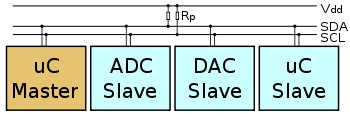
\includegraphics[width=0.3\columnwidth]{img/i2c-bus.png}
% 	\caption{Bus \IIC}%
% 	\label{fig:iic-bus}
% \end{wrapfigure}


% %% %%%%%%%%%%%%%%%%%%%%%%%%%%%%%%%%%%%%%%%%%%%%%%%%%%%%%%%%%%
% intro.tex
%
% Author:  Mauricio Matamoros
% License: MIT
%
% %% %%%%%%%%%%%%%%%%%%%%%%%%%%%%%%%%%%%%%%%%%%%%%%%%%%%%%%%%%%

%!TEX root = ../practica.tex
%!TEX root = ../references.bib

\subsection{MicroPython}%
\label{sec:uPy}

% The use of the Python language for controlling hardware has been around for some time. Users of the Raspberry Pi, pcDuino, and other low-cost computers and similar boards have had the advantage of using Python for controlling hardware. In this case, they used full versions of the Python programming language on the native Linux-based operating system. While these boards made it possible for those who wanted to develop electronics projects, it required users to buy the board as well as peripherals like a keyboard, mouse, and monitor. Not only that, but users also had to learn the operating system. For those not used to Linux, this can be a challenge in and of itself.

% The vision for MicroPython was to combine the simplicity of learning Python with the low cost and ease of use of microcontroller boards, which would permit a lot more people to work with electronics for art and science projects. Beginners would not have to learn a new operating system or learn one of the more complex programming languages.

Creado por Damien P. George y Paul Sokolovsky (entre otros),
MicroPython fue diseñado para ser una versión ligera y eficiente del lenguaje Python 3 instalable en un pequeño microcontrolador.
Dado que Python es un lenguaje interpretado y, por lo tanto, en general más lento que los lenguajes compilados (véase~\Cref{sec:uPy-interpreter}), MicroPython fue diseñado para ser lo más eficiente posible para que pueda ejecutarse en microcontroladores que normalmente son más lentos y tienen mucha menos memoria que una computadora personal típica~\Citep{bell2022MicroPython,bell2022}.

Otro aspecto es que las tarjetas microcontroladores como Arduino requieren que el código sea compilado en otra computadora para producir un código objeto ejecutable que debe ser cargado en dicha tarjeta.
En contraste, dado que MicroPython es un intérprete ejecutándose directamente en el hardware, puede prescindirse del paso intermedio de compilación:
¡se puede ejecutar el código fuente directamente en el hardware!
Esto permite a los fabricantes de hardware construir tarjetas pequeñas y económicas con MicroPython embebido en el chip y que puedan ejecutar virtualmente cualquier programa tanto en la fase de desarrollo como en la de producción~\Citep{bell2022MicroPython,bell2022}.

MicroPython permite crear programas simples, eficientemente especificados y fáciles de entender.
Además, incluye las siguientes características~\Citep{bell2022MicroPython,bell2022}:

\begin{itemize}[nosep]
	\item \textbf{Intérprete interactivo:} MicroPython habilita en la tarjeta física una consola interactiva especial a la que puede acceder conectándose via USB. % CHKTEX 13

	\item \textbf{Bibliotecas estándar de Python:} MicroPython es compatible con muchas de las bibliotecas estándar de Python.
	En general, uno puede confiar en que alrededor del del 80\% de las bibliotecas más utilizadas estarán disponibles.

	\item \textbf{Bibliotecas a nivel de hardware:} MicroPython tiene bibliotecas integradas que le permiten acceder al hardware directamente para encender o apagar pines, leer datos analógicos, leer datos digitales, controlar hardware (PWM) y más.

	\item \textbf{Extensible:} MicroPython también es extensible.
	Ésta es una gran característica para usuarios avanzados que necesitan implementar alguna biblioteca compleja de bajo nivel (en C/C++) e incluir la nueva biblioteca en MicroPython.
\end{itemize}

La mayor limitación de MicroPython  deriva de su facilidad de uso:
aunque MicroPython está altamente optimizado el código se interpreta sobre la marcha lo que agrega una penalización de desempeño y memoria por parte del intérprete.
Esto significa que los proyectos que requieren un alto grado de precisión, un muestreo de datos a alta frecuencia, o comunicaciones a alta velocidad (por ejemplo USB), pueden no ejecutarse lo suficientemente rápido.
Estos problemas suelen superarse con el uso de bibliotecas en C/C++ optimizadas para manejar la comunicación de bajo nivel.
Por otro lado, MicroPython también requiere de un poco más de memoria que el código nativo.
Normalmente, esto no es un problema, aunque debe tomarse en cuenta si el programa va a extenderse con características nuevas.
Los programas más grandes que usan muchas bibliotecas podrían consumir más memoria de la disponible.
Finalmente, como se mencionó anteriormente, MicroPython no implementa todas las funciones de todas las bibliotecas de Python 3~\Citep{bell2022MicroPython,bell2022}.



\subsection{Lenguajes compilados \textsuperscript{v}/\textsubscript{s} lenguajes interpretados}%
\label{sec:uPy-interpreter}
Los lenguajes compilados requieren de un programa externo llamado compilador para convertir el código fuente de una forma legible por humanos a una forma ejecutable binaria que pueda ser entendido y ejecutado con máxima eficiencia por el procesador.
Por otro lado, los lenguajes interpretados no se compilan, sino que se evalúan línea a línea sobre la marcha con un programa llamado intérprete.
Python 3 proporciona un ejecutable de Python que es a la vez un intérprete y una consola que le permite ejecutar el código a medida que se escribe.

Por lo tanto, los lenguajes compilados son mucho más rápidos que los lenguajes interpretados porque el código está preparado (y optimizado) para su ejecución en el microprocesador sin requerir de pasos intermedio en tiempo real para procesar el código antes de la ejecución.

% %% %%%%%%%%%%%%%%%%%%%%%%%%%%%%%%%%%%%%%%%%%%%%%%%%%%%%%%%%%%
% intro-adc.tex
%
% Author:  Mauricio Matamoros
% License: MIT
%
% %% %%%%%%%%%%%%%%%%%%%%%%%%%%%%%%%%%%%%%%%%%%%%%%%%%%%%%%%%%%
% CHKTEX-FILE 1
% CHKTEX-FILE 46
%!TEX root = ../practica.tex
%!TEX root = ../references.bib

\subsection{Convertidor Analógico---Digital}%
\label{sec:intro-adc}
Para leer la señal del LM35 se requiere de un Convertidor Analógico Digital o ADC (por sus siglas en inglés: \emph{Digital-Analog Converter}).
Un ADC se elige con base en dos factores clave: su precisión y su tiempo de muestreo.
Debido a que la aplicación del ADC será convertir mediciones de temperatura y los cambios de temperatura son muy lentos,\footnotemark{} puede obviarse el tiempo de muestreo.
En cuanto a la precisión, los convertidores A/D más comunes son de 8 y 10 bits, de los cuales ha de elegirse uno.

La precisión del ADC se calcula tomando en cuenta el rango de operación y la precisión del componente analógico a discretizar.
El LM35 tiene un rango de \degreesC{205}, una diferencial de voltaje $\Delta{}V=10mV/^{o}C$ y una precisión máxima de \degreesC{0.5}, por lo que el sensor entregará un máximo de 2.5V respecto al voltaje de referencia del mismo, con incrementos de 5mV.
Debido a que 256 valores para un rango de \degreesC{205} en incrementos de \degreesC{0.5} (es decir 410 valores) es claramente insuficiente para este sensor, por lo que será conveniente utilizar un convertidor A/D de 10 bits.

Un ADC típico de 12 bits convertirá las señales analógicas entre voltajes de referencia $V_{Ref-}$ y $V_{Ref+}$ como un entero con valores entre 0 y 4096, interpretando los valores $V_{Ref-}$ como 0 lógico y $V_{Ref+}$ como 4096 de manera aproximadamente lineal.
El decir, la lectura obtenida es directamente proporcional al voltaje dentro del rango, estimable mediante la fórmula:

\begin{equation}
V_{out}= value \times \frac{ V_{Ref+} - V_{Ref-} }{ 4096 }
\end{equation}

En una configuración simple, $V_{Ref-}$ y $V_{Ref+}$ se conectan internamente dentro del RP2040 a tierra y V\textsubscript{CC} respectivamente. Esto simplifica la fórmula como:

\begin{equation}
V_{out}= value \times \frac{ 5V }{ 4096 } = value \times 1.22mV
\end{equation}

En lo concerniente al RP040, éste incorpora un convertidor analógico-digital de 12 bits con soporte para voltaje de referencia $V_{Ref+}$, denominado \emph{ADC\_VREF} según las especificaciones del mismo~\Citep{RP2040datasheet}.
Considerando que el LM35 en rango completo entrega hasta 2.05V ($10mV\times (150 - -55) = 2.05V$) la mayor parte de los 4096 valores jamás serán ocupados.
Por este motivo, conviene sacar partido del pin de voltaje de referencia \emph{ADC\_VREF} del RP2040 mediante un divisor de voltaje (véase~\Cref{fig:lm35-pico}).
En consecuencia, el pin \emph{ADC\_VREF} requerirá de un divisor de voltaje con salida de 2.73V tal como se muestra en la~\Cref{fig:lm35-pico} para dar mayor precisión al convertidor A/D.

\begin{figure}
	\centering
	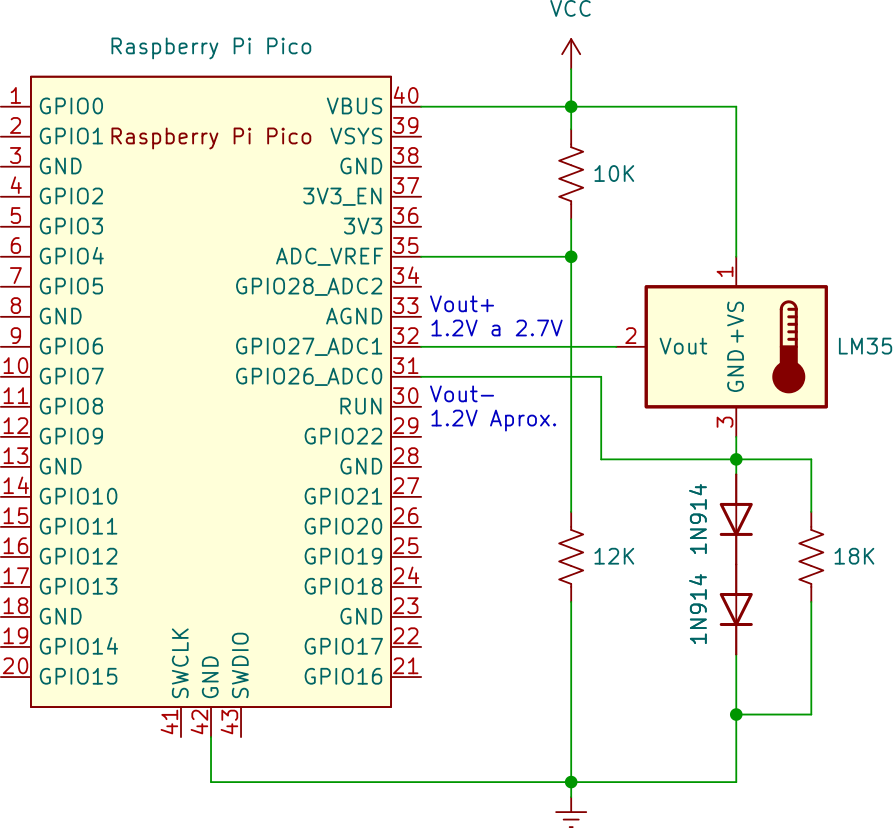
\includegraphics[width=\textwidth,height=7cm,keepaspectratio]{img/lm35-pico.png}
	\caption{Circuito medidor de temperatura LM35 con el RP2040}
	\label{fig:lm35-pico} % chktex 24
\end{figure}

Con esta nueva configuración, se puede calcular de nueva cuenta la precisión del sensor digital una vez decodificado el valor analógico leído del LM35 dividiendo los 2.73V de referencia entre los 4096 valores posibles que entrega el ADC como sigue:

\begin{equation}
\Delta V = \frac{ 2.73V }{ 4096 } =  666.5\times10^{-6}V = 667\mu{}V
\end{equation}

Debido a que la resolución máxima del sensor LM35 determinada por su factor de incertidumbre es de \degreesC{0.5} equivalentes a 0.005V, ambas configuraciones (con y sin el divisor de voltaje) serán adecuadas para operar al sensor.

% %% %%%%%%%%%%%%%%%%%%%%%%%%%%%%%%%%%%%%%%%%%%%%%%%%%%%%%%%%%%
% intro-lm35.tex
%
% Author:  Mauricio Matamoros
% License: MIT
%
% %% %%%%%%%%%%%%%%%%%%%%%%%%%%%%%%%%%%%%%%%%%%%%%%%%%%%%%%%%%%

%!TEX root = ../practica.tex
%!TEX root = ../references.bib


\subsection{Thonny}%
\label{sec:intro-thonny}

Thonny es un IDE\footnote{Entorno de desarrollo integrado, por sus siglas en inglés \emph{Integrated Development Environment}}
de código abierto
para Python desarrollado por la Universidad de Tartu, Estonia, pensado para ser amigable con el principiante.
Además de las capacidades estándar de construcción y ejecución de programas, cuenta con un soporte extendido para animación de programas,
permitiendo ilustrar los conceptos de variables, control de flujo, evaluacíón de expresiones, llamada a funciones, recursión, referencias y montículos, objetos (incluyendo clases y funciones como valores), datos compuestos (listas, diccionarios y conjuntos) y operaciones de entrada/salida sobre archivos~\Citep{annamaa2015a,annamaa2015b}.

Thonny puede llevar registro de las acciones del usuario con suficiente detalle para reproducir el proceso de elaboración de un programa, permitiéndole a los estudiantes elegir el nivel de detalle con el que desean analizar la reproducción~\Citep{annamaa2015a,annamaa2015b}.

Una de las ventajas de Thonny sobre cualquier otro editor de Python es que, a partir de la versión 4.0, incluye soporte para interactuar con varios  microcontroladores como el RP2040, el ESP32 y el ESP8266; todos de amplia difusión en el mercado.
Además, Thonny permite realizar operaciones en el sistema de archivos virtual del RP2040 (MicroPython convierte el RP2040 en una suerte de memoria USB de unos cuantos kB).
Para este fin, basta con contectar la tarjeta controladora a la PC, iniciar Thonny y seleccionar las opciones \emph{View} y \emph{Files}.
De igual manera Thony permite copiar archivos de y a la tarjeta controladora para ser utilizados por MicroPython~\cite{bell2022MicroPython,bell2022}.

\begin{figure}[H]
	\centering%
	\includegraphics[width=\columnwidth,height=8cm,keepaspectratio]{img/thonny-files.png} %CHKTEX 8
	\caption{Thonny permite visualizar, crear, copiar, cortar, pegar y, en general, manupular archivos dentro del RP2040.}
	\label{fig:thonny} %CHKTEX 24
\end{figure}

